\documentclass[10pt,twocolumn]{article}

\usepackage[letterpaper,margin=0.75in,columnsep=0.22in]{geometry}
\usepackage{times}
\usepackage{microtype}
\usepackage{graphicx}
\usepackage{booktabs}
\usepackage{amsmath,amssymb,amsfonts}
\usepackage{xcolor}
\usepackage{caption}
\usepackage{subcaption}
\usepackage[numbers,sort&compress]{natbib}
\usepackage[hidelinks]{hyperref}

\graphicspath{{figures/}}

\captionsetup{font=small,labelfont=bf,skip=4pt}
\captionsetup[subfigure]{font=scriptsize,skip=1pt,labelfont=bf}
\setlength{\textfloatsep}{8pt plus 2pt minus 2pt}
\setlength{\floatsep}{6pt plus 2pt minus 2pt}
\setlength{\intextsep}{8pt plus 2pt minus 2pt}
\setlength{\abovecaptionskip}{4pt}
\setlength{\belowcaptionskip}{0pt}
\setlength{\abovedisplayskip}{6pt}
\setlength{\belowdisplayskip}{6pt}
\setlength{\parskip}{0pt}
\setlength{\parindent}{11pt}
\renewcommand{\topfraction}{0.92}
\renewcommand{\bottomfraction}{0.85}
\renewcommand{\textfraction}{0.08}
\renewcommand{\floatpagefraction}{0.82}

\title{\vspace{-0.5em}GALA-WM: Residual Action-Conditioned Latent Dynamics\\for Human Motion World Models}
\author{Anonymous\\[2pt]
\small\textbf{Code:} \url{https://github.com/yanghhx/gala-motion}}
\date{}

\begin{document}
\maketitle
\vspace{-0.9em}

\begin{abstract}
\vspace{-0.2em}
The ability to predict future poses given control actions is fundamental if human motion is to serve as a simulator, yet most motion systems remain open-loop generators.
Synthesizers such as the Motion Diffusion Model and MoMask emit a full clip with no counterfactual rollout; pixel-level world models reconstruct visual dynamics at high cost; humanoid controllers assume a physics API that motion-capture datasets do not provide.
We present GALA-WM, an action-conditioned latent world model for human locomotion.
Our key insight is that a frozen motion tokenizer already yields a compact, near-lossless latent, so simulation reduces to learning residual dynamics that are modulated and gated by explicit root commands---null actions then collapse toward a copy-last baseline, making control necessary rather than optional.
GALA-WM encodes HumanML3D poses with a frozen graph-aware VAE, predicts residual latent transitions with a FiLM-conditioned Transformer, and plans with latent CEM following the DINO-WM protocol.
Extensive experiments on HumanML3D show that GALA-WM reduces 1.6\,s MPJPE from 76.7\,mm (copy-last) to 53.0\,mm and raises goal-reaching success from 50\% (hold) to 73.9\%, yielding a locomotion simulator rather than another text-conditioned synthesizer.
Code is available at \url{https://github.com/yanghhx/gala-motion}.
\vspace{-0.3em}
\end{abstract}

\section{Introduction}

World models answer ``what happens if I act''~\cite{ha2018world,hafner2025dreamerv3,lecun2022path}.
Closed-loop benchmarks such as World-in-World~\cite{zhang2026worldinworld} show that visual fidelity does not imply task utility: a model that looks realistic can still be a poor simulator.
Human motion generation has the same gap.
MDM~\cite{tevet2023mdm}, TEMOS~\cite{petrovich2022temos}, MotionDiffuse~\cite{zhang2024motiondiffuse}, MLD~\cite{chen2023executing}, and MoMask~\cite{guo2024momask} map text to a full clip.
They have no action interface, no counterfactual rollout, and no planner.

We freeze a GALA tokenizer on HumanML3D~\cite{guo2022humanml3d} and train only dynamics (Fig.~\ref{fig:arch}), following the DINO-WM recipe of a frozen encoder plus a latent transition plus CEM~\cite{zhou2024dinowm}.
The claim is narrow and testable: residual action-conditioned latents should beat copy-last, zero-action, and shuffled-action baselines on multi-step MPJPE, fork under reversed locomotion, and improve CEM over a hold planner.

\paragraph{Contributions.}
(1)~Recast a text-to-motion VAE as a DINO-WM-style simulator, with all forward computation in a $256$-D motion latent.
(2)~FiLM modulation plus an action gate so $a{=}0$ collapses toward copy-last, widening the GT--zero gap.
(3)~Closed-loop diagnostics---horizon MPJPE, action swap, CEM vs.\ hold---rather than FID~\cite{ebert2018visual,hafner2019planet,zhou2024dinowm}.

\begin{figure*}[t]
\centering
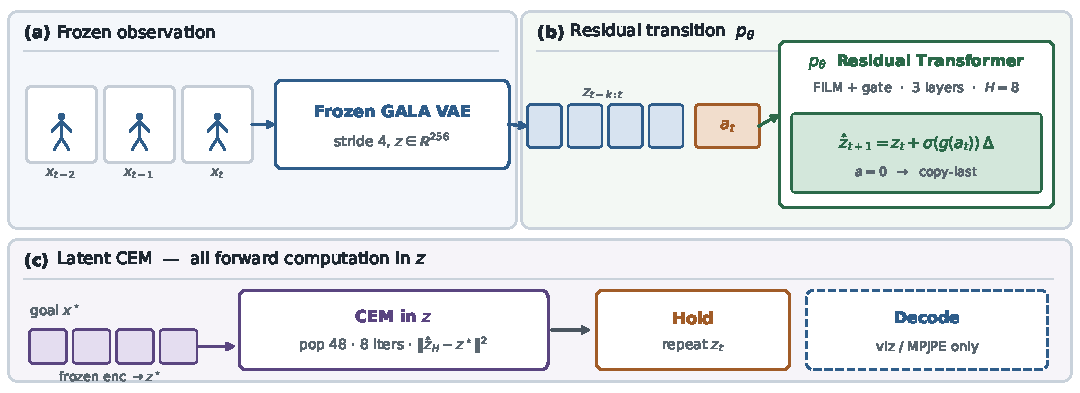
\includegraphics[width=\textwidth]{fig1_architecture.pdf}
\caption{Overview of GALA-WM, drawn after DINO-WM~\cite{zhou2024dinowm} (Fig.~2) and MLD~\cite{chen2023executing}.
Given poses $x_{t-k:t}$, we optimize actions $a_{t:H-1}$ to reduce the predicted latent loss to a goal $x^\star$.
All forward computation is done in $z$.
\textbf{(a)}~A frozen graph-aware VAE maps HumanML3D poses to $256$-D latents.
\textbf{(b)}~Residual transition $p_\theta$: a FiLM-conditioned Transformer, gated by the action, predicts $\hat z_{t+1}=z_t+\sigma(g(a_t))\Delta$.
\textbf{(c)}~Latent CEM (and a hold baseline) plan in $z$; the decoder is used only for visualization and MPJPE.}
\label{fig:arch}
\end{figure*}

\section{Related work}

\paragraph{Latent world models.}
Dreamer, PlaNet, and MuZero~\cite{hafner2020dreamerv2,hafner2025dreamerv3,hafner2019planet,schrittwieser2020muzero}, TD-MPC~\cite{hansen2022tdmpc,hansen2024tdmpc2}, and transformer world models~\cite{seo2023masked,micheli2023transformers,robine2023transformer} learn $p(z_{t+1}\mid z_{\le t},a_t)$.
DINO-WM~\cite{zhou2024dinowm} freezes DINOv2~\cite{oquab2024dinov2} and plans with CEM---the architectural and planner template we follow.
DIAMOND, Genie, and Cosmos~\cite{alonso2024diamond,bruce2024genie,nvidia2025cosmos} target pixels; we stay in a $256$-D motion latent~\cite{assran2023vjepa,moerland2023modelbased}.
Copy-last, zero/shuffle action, and hold/CEM are diagnostic protocols from this literature~\cite{mathieu2016video,oh2015action,finn2016unsupervised,rubinstein1999cem}, not reimplementations of MDM or DreamerV3.

\paragraph{Motion and humanoids.}
Puppeteer and Humanoid World Models~\cite{hansen2024puppeteer,ali2025hwm} and physics controllers~\cite{peng2018deepmimic,won2022physics,ling2020character,luo2023perpetual,rempe2021humor,yuan2023physdiff} need a simulator API.
Text-to-motion models~\cite{tevet2023mdm,chen2023executing,zhang2023remodiffuse,jiang2024motiongpt,shafir2024human} optimize $p(x\mid\text{text})$.
We use HumanML3D locomotion~\cite{guo2022humanml3d,mahmood2019amass,punnakkal2021babel,loper2015smpl} as a cheaper proxy.

\section{Method}

Frozen GALA maps $x_{1:T}\!\in\!\mathbb{R}^{T\times 263}$ to $\mu\!\in\!\mathbb{R}^{L\times 256}$~\cite{kingma2014vae,loper2015smpl} (Fig.~\ref{fig:arch}a).
Action $a_\ell\in\mathbb{R}^{4}$ is the mean of the root channels $(\dot\psi,v_x,v_z,h)$ over the four corresponding frames.
Residual dynamics (Fig.~\ref{fig:arch}b) are
\begin{equation}
\hat\mu_{t+1}=\mu_t+\sigma\bigl(g(a_t)\bigr)\,\Delta(\mu_{t-k:t},a_t),
\end{equation}
with FiLM~\cite{perez2018film} on every history token and a 3-layer Transformer~\cite{vaswani2017attention,dosovitskiy2021vit}.
When $a{=}0$, the gate collapses the residual toward copy-last, so control is necessary rather than optional.
We train with an $H{=}8$ unroll plus a decoded pose loss.

CEM (Fig.~\ref{fig:arch}c) uses population 48, 8 iterations, and cost $\|\hat\mu_H-\mu^\star\|^2+0.35\cdot\mathrm{mean}_h\|\hat\mu_h-\mu^\star\|^2$~\cite{rubinstein1999cem,zhou2024dinowm}; hold repeats $z_t$.
Evaluation uses 92 validation clips, horizons $\{1,4,8\}$ ($\approx 0.2/0.8/1.6$\,s), denormalized MPJPE, a planar-velocity swap, and CEM success if MPJPE $<80$\,mm and root XY $<0.5$\,m.

\section{Experiments}

\textbf{Setup.} Official HumanML3D~\cite{guo2022humanml3d}; batch 8, AdamW $2{\times}10^{-4}$, bf16, RTX 4060.
Unfixed predicts an absolute next latent in one step; v1 is residual; v2 adds FiLM, the action gate, and an $H{=}8$ unroll.

\subsection{Open-loop prediction}
v2 with ground-truth actions is lowest at every horizon (Fig.~\ref{fig:quant}a, Table~\ref{tab:main}); shuffled actions exceed copy-last.
FiLM and the gate push zero/shuffle toward copy-last while GT stays low (Fig.~\ref{fig:quant}b): at horizon 8, v2 improves 23.7\,mm over copy-last and widens the GT--zero gap from 10\,mm (v1) to 22\,mm.

\begin{table}[t]
\centering
\caption{Main results on HumanML3D val ($n{=}92$). MPJPE in mm; planning on the right.}
\label{tab:main}
\scriptsize
\setlength{\tabcolsep}{3.2pt}
\begin{tabular}{@{}lcccccc@{}}
\toprule
Method & @1 & @4 & @8 & $\Delta$XY & CEM\% & Hold\% \\
\midrule
Copy-last / Hold & 35.8 & 60.6 & 76.7 & -- & -- & 50 \\
Unfixed & 29.7 & 51.9 & 74.1 & 0.46 & 54.3 & 50 \\
v1 residual & 21.5 & 39.9 & 58.2 & 0.58 & 65.2$^\dagger$ & 50 \\
\textbf{v2 FiLM/gate} & \textbf{21.6} & \textbf{39.0} & \textbf{53.0} & \textbf{0.62} & \textbf{73.9} & 50 \\
\midrule
v2 + zero $a$ & 29.3 & 53.5 & 75.1 & & & \\
v2 + shuffle $a$ & 43.9 & 68.6 & 89.9 & & & \\
\bottomrule
\end{tabular}\\[1pt]
{\scriptsize $^\dagger$Weak CEM 65.2\%; strong CEM on v1 reaches 71.7\% / 76.8\,mm.}
\end{table}

\begin{figure*}[t]
\centering
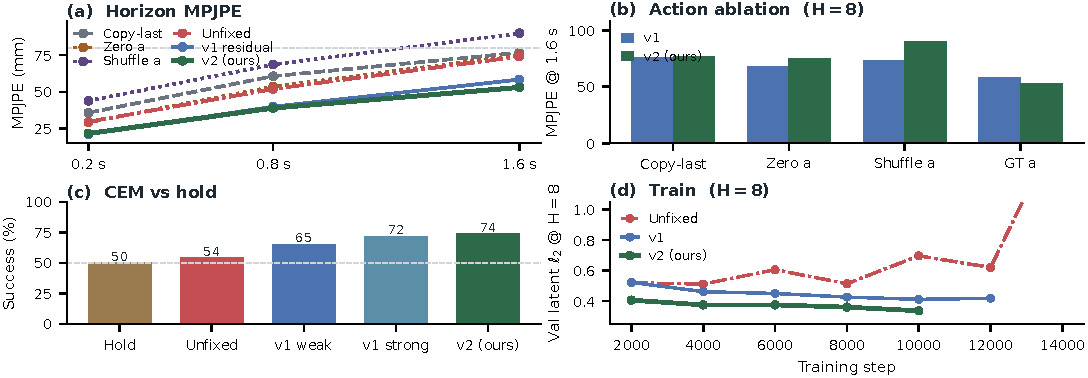
\includegraphics[width=\textwidth]{fig_quant.pdf}
\caption{Quantitative diagnostics on HumanML3D val ($n{=}92$).
\textbf{(a)}~Open-loop MPJPE vs.\ horizon.
\textbf{(b)}~Action ablation at $H{=}8$: FiLM+gate pushes zero/shuffle toward copy-last while GT stays low.
\textbf{(c)}~Latent CEM vs.\ hold (success if MPJPE $<80$\,mm and root XY $<0.5$\,m).
\textbf{(d)}~Online val latent $\ell_2$ at $H{=}8$; unfixed diverges.}
\label{fig:quant}
\end{figure*}

\subsection{Planning and qualitative results}
CEM reaches 73.9\% success versus 50\% for hold (Fig.~\ref{fig:quant}c, Table~\ref{tab:main}).
Fig.~\ref{fig:qual} shows open-loop skeletons, CEM versus hold, and root trajectories; the decoder is used only for visualization.

\begin{figure*}[t]
\centering
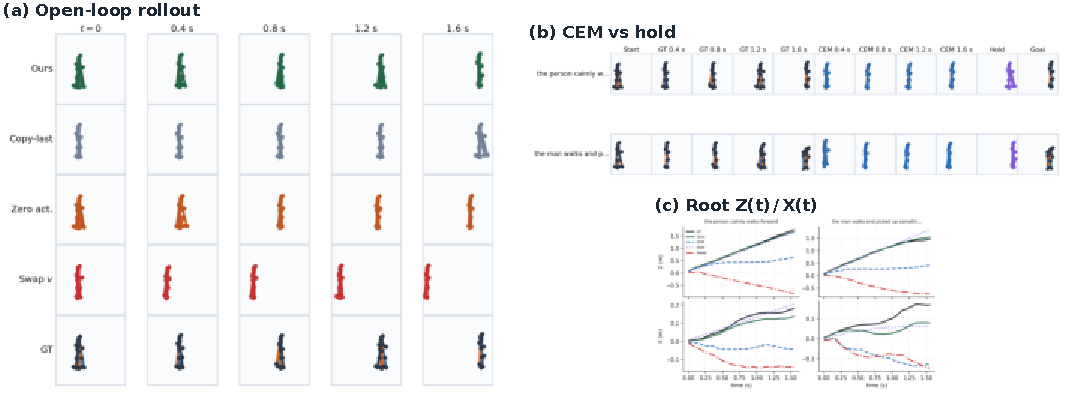
\includegraphics[width=\textwidth]{fig_qual.pdf}
\caption{Qualitative results.
\textbf{(a)}~Open-loop rollout of v2 against copy-last, zero action, velocity swap, and GT.
\textbf{(b)}~CEM vs.\ hold on two locomotion goals.
\textbf{(c)}~Integrated root $Z(t)/X(t)$; swap forks planar velocity, CEM tracks the goal more tightly than hold.}
\label{fig:qual}
\end{figure*}

\section{Limitations and conclusion}

Actions are locomotion-centric; we do not transfer to physics simulators~\cite{hansen2024puppeteer,zhang2026worldinworld}; CEM still fails on 26\% of goals; validation is 92 clips, one seed.
Residual, action-gated dynamics on a frozen motion VAE nevertheless yield a DINO-WM-style simulator that beats protocol baselines on prediction and planning~\cite{zhou2024dinowm,black2024pi0,lecun2022path,sutton2018rl}.

\bibliographystyle{unsrtnat}
\bibliography{references}

\end{document}
